Transformers operate on sequences of data $(x_{k})_{k=1}^n$, where $x_{k} \in \mathbb R^d$.
In the literature the elements of the input sequence are commonly referred to as tokens.
Central to Transfomer models is the so-called attention mechanism.
The tokens $x_k$ are embedded into three different subspaces using linear mappings $Q, K, V \in \mathbb R^{d', d}$.
The mappings $Q$ and $K$ are used to compute the attention scores among the members of the sequence,
measuring the level of relevance of their respective information for each other

    \begin{equation} \label{eq:sa1}
        A_{ij} = \frac{\text{exp}(x_{i}^T K^T Q x_{j})}{\sum_{k = 1}^n \text{exp}(x_{k}^T K^T Q x_{j})} ~.
    \end{equation}

The outputs are then computed for all $j=1, ..., n$ by 

    \begin{equation} \label{eq:sa2}
        y_{j} = \sum_{i=1}^n A_{ij} V x_{i} ~.
    \end{equation}

Note that by construction for all $j = 1,..., n$ holds

    $$ \sum_{i=1}^n A_{ij} = 1 ~. $$

\begin{definition}[Self-Attention]
    Let $Q, K, V \in \mathbb R^{d', d}$.
    The operation described in equations (\ref{eq:sa1}), (\ref{eq:sa2}) 

        $$ \text{SA}: \mathbb R^{d} \times ... \times R^{d} \to R^{d} \times ... \times R^{d} ~, ~~ \text{SA} (Q, K, V)(x_1, ..., x_k) = [y_1, ..., y_k] ~, $$

    is called self-attention.
\end{definition}

To increase the expressiveness of Transformer models multiple self-attention mappings, 
called heads in the literature, are used in parallel to process the input sequence.

\begin{definition}[Multi Headed Self-Attention]
    Let $Q_h, K_h, V_h \in \mathbb R^{d', d}$ for $h= 1,..., H$ and let $Q = (Q_1, ..., Q_H), K = (K_1, ..., K_H), V = (V_1, ..., V_H)$.
    The operation

        $$ \text{MSA}(Q, K, V) = [\text{SA}(Q_1, K_1, V_1), ..., \text{SA}(Q_H, K_H, V_H)] ~, $$

    is called multi headed self-attention.
\end{definition}

\begin{figure}[h!]
    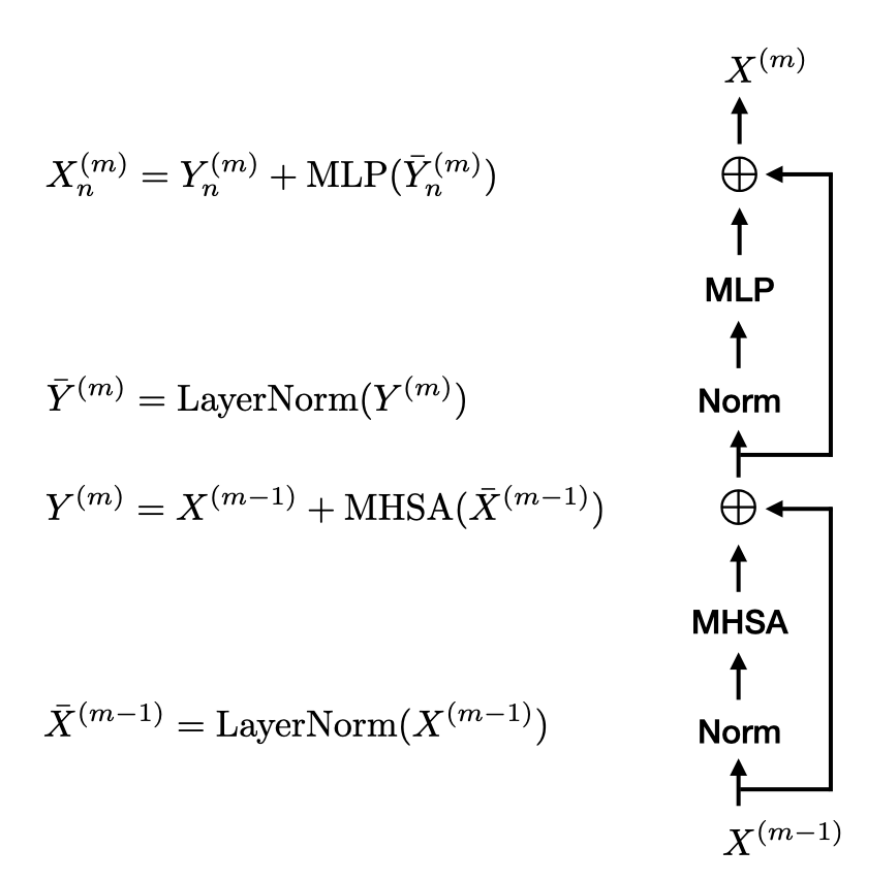
\includegraphics[width=0.6\textwidth]{models/preliminaries/imgs/transformer-block.png}
    \caption{Image taken from \cite{turnerIntroductionTransformers2024}, Transformer Block architecture.}
    \label{fig:transformer_block}
\end{figure}

In order to refer to the architecture,
thats is Multi Headed Self-Attention with dimension $d \in \mathbb N$ and number of heads $H \in \mathbb N$,
whose weights are not fixed but subject to optimization, 
we write $\text{MSA}(d, H)$.

Given a numer of heads $H \in \mathbb N$ generally the embedding dimension of each head is chosen as $\frac{d}{H}$.

Another key ingridient for Transformer models is layer normalization.

\begin{definition}[Layer Normalization]
    Let $\gamma \in \mathbb R$ and $\beta \in \mathbb R^d$. The operation given by

        $$\text{LN} : \mathbb R^d \to \mathbb R^d ~, ~~ 
        \text{LN}(x) = \gamma \bar{x} + \beta 
        \text{ where } \bar{x}_{ki} = \frac{1}{\sqrt{\text{var}(x_{k})}} (x_{ki} - \sum_{j=1}^d x_{kj})$$

    is caled layer normalization.
\end{definition}

Typically Multi Headed Self-Attention is used in transfomer blocks,
the architecture is outlined in figure \ref{fig:transformer_block}.

First layer normalization is applied to the inputs before the Multi Headed Self-Attention is being performed.
The input is then added back to the outputs via a residual connection.
The intermediate throughputs then undergo a second round of layer normalization, 
the tokens are then processed individually by a neural network.
Mathematically this can be summarized by

\begin{equation*}
    \text{TransfomerBlock} = R \big( \Phi \circ \text{LN} \big) \circ R \big( \text{MSA}(d, H) \circ \text{LN} \big)
\end{equation*}

where $\Phi: \mathbb{R}^d \to \mathbb{R}^d$ is some neural network, typically with only a few number of layers.